\chapter{Preliminaries}\label{c-Prelim}

\section{Taylor Polynomials}
We want an easier way of calculating a difficult function, $f(x)$.  To this end we want to find a function that is similar to our original that we can calculate.  Taylor polynomials, $p_n(x)$\footnote{The subscript $n$ tells the highest power of the polynomial, i.e. $x^n$.}, are one such type of functions with an easy calculation and intuition.  To find the Taylor polynomials we match the derivatives of the two polynomials at a particular point.  We are in essence enforcing a smoothness criterion at the point of interest, say $x=a$.
\beqn
p_n'(a) &=& f'(a) \\
p_n''(a) &=& f''(a) \\
&\vdots & \\
p_n^{(n)}(a) &=& f^{(n)}(a)
\eeqn
Thus the general expression for the Taylor series is
\beqn
p_n(x) &=& f(a)+(x-a)f'(a)+\frac{(x-a)^2}{2!}f''(a)+\ldots+\frac{(x-a)^n}{n!}f^{(n)}(a) \\
&=& \sum_{k=0}^{n}\frac{(x-a)^k}{k!}f^{(k)}(a)
\eeqn

\textbf{Example}

Problem 1.1-3(c)
\beqn
f(x) &=& \sqrt{1+x} \\
f(0) &=& \sqrt{1+0}=1 \\
f'(0) &=& \frac{1}{2\sqrt{1+0}}=\frac{1}{2} \\
f''(0) &=& \frac{-1}{4(\sqrt{1+0})^3}=\frac{-1}{4} \\
f''(0) &=& \frac{3}{8(\sqrt{1+0})^5}=\frac{3}{8} \\
f^{(k)}(0) &=& \frac{(-1)^{k-1}(2k-3)}{2^k}
\eeqn

\begin{figure}
  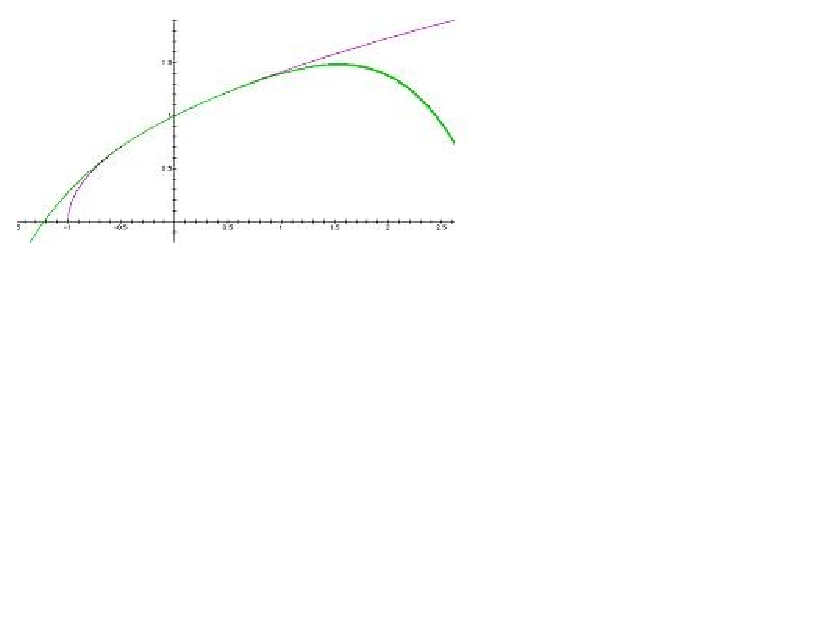
\includegraphics[width=4in]{taylorfit.eps}\\
  \caption{Taylor polynomial and $\sqrt{1+x}$}\label{f-taylor1}
\end{figure}



\textbf{Example}

Problem 1.1-8
\beqn
f(x) &=& \frac{\log(1+x)}{x} \\
&\approx & \frac{\sum_{k=1}^n\frac{(-1)^{k-1}}{k}x^k}{x} \\
&=& \sum_{k=1}^n\frac{(-1)^{k-1}}{k}x^{k-1} \\
f(0) &\approx & 1
\eeqn


\section{Remainder}
The Taylor Series obviously has errors in its approximation.  If the
original function is in $C_{n+1}$ on the interval $\alpha\leq x\leq\beta$ (with $a$ in the
interval) then the remainder (or error) is given by
\beqn
R_n(x) &=& f(x)-p_n(x) \\
&=& \frac{(x-a)^{n+1}}{(n+1)!}f^{(n+1)}(c_x)
\eeqn
with $c_x$ between $a$ and $x$.  To get an error bound we assume that $c_x$ is the worst possible.

\textbf{Example}

Problem 1.2-3(a)
In this case $n=1$ so the worst case would be if $\cos(c_x)=-1$ were $-1$.
\beqn
R_n(x)=\frac{x^{2(1)+1}}{(2(1)+1)!}=\frac{x^3}{6}\leq\frac{\pi^3}{324}<0.081
\eeqn

\textbf{Example}

Prove problem 8.


\section{Evaluating Polynomials}

Consider the polynomial
\beqn
y=a_nx^n+a_{n-1}x^{n-1}+\ldots+a_1x+a_0
\eeqn

\subsection{Straightforward}
The obvious way is to calculate each term separately,
\beqn
a_kx^k=a_k*x*x*...*x
\eeqn
This takes $k$ multiplications for a monomial of size $k$, so for a polynomial with monomials up to size $n$ it would take $\frac{n(n+1)}{2}$ multiplications.

\subsection{Storing}
Calculate $x2=x*x$, $x3=x*x2$, etc. This takes $2n-1$ multiplications.  This is much better that the straightforward way.  We can even do this without having to store each intermediate result by using a temporary variable.  Still it is not the best.

\subsection{Nesting}

Rewrite the polynomial as
\beqn
y&=&a_nx^n+a_{n-1}x^{n-1}+\ldots+a_1x+a_0 \\
&=&((\ldots(((a_n)x+a_{n-1})x+a_{n-2})\ldots)x+a_1)x+a_0.
\eeqn
This can be done as
\beqn
b_n&=&a_n \\
b_{n-1}&=&b_nx+a_{n-1} \\
b_{n-2}&=&b_{n-1}x+a_{n-2} \\
&\vdots & \\
b_1&=&b_2x+a_1 \\
b_0&=&b_1x+a_0
\eeqn
Each step takes 1 multiply so this method takes only n multiplications.  The real savings come when you have to calculate a large polynomial many times.  Another interesting thing is this is a more accurate method,  see Fig~\ref{f-polyeval}, where the dark blue line is the nested multiplication method.  Note on the right side both methods are equally good (or bad in my opinion), but on the right the nested multiplication technique shows marked improvement in accuracy.  Not bad for less work.


\begin{figure}[h]
  % Requires \usepackage{graphicx}
  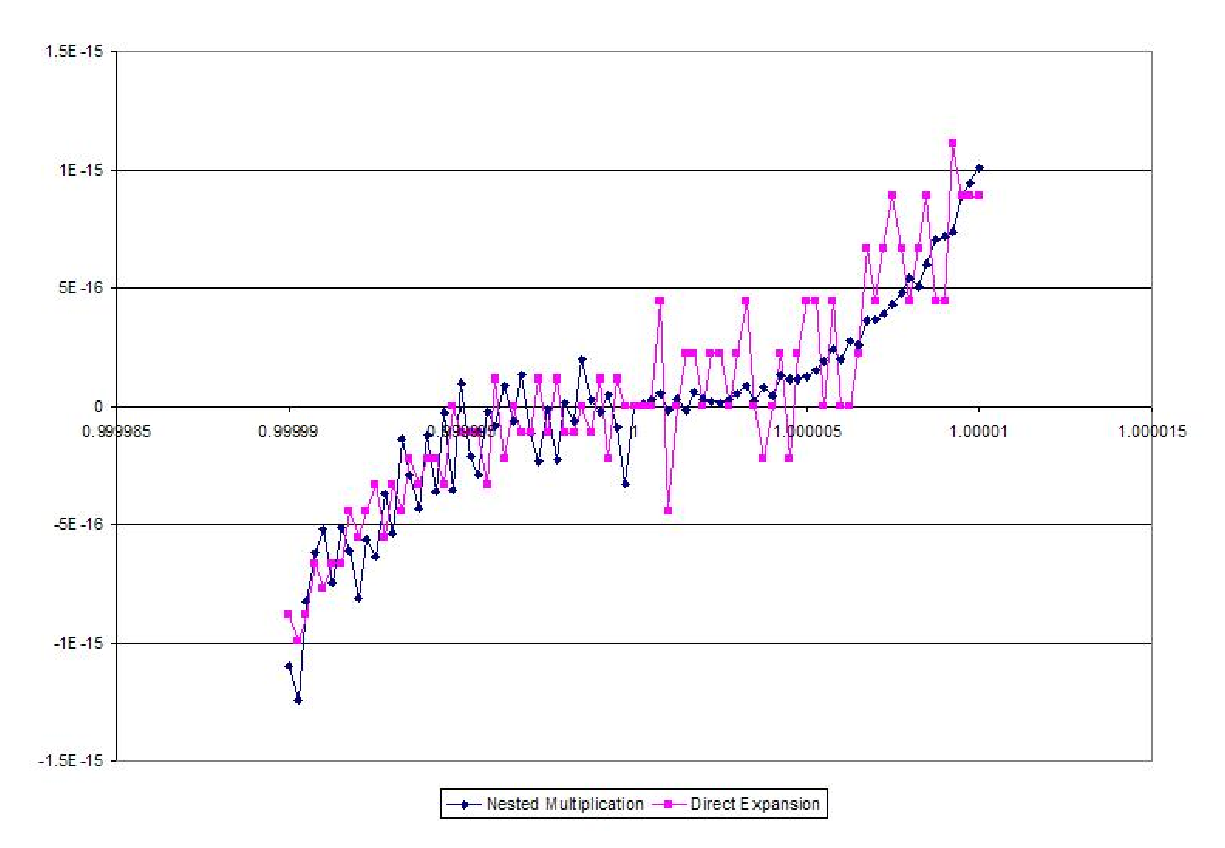
\includegraphics[width=4in]{cubicpoly.eps}\\
  \caption{Close-up Look at Resulting Values of Two Evaluation Methods for $y=x^3-3x^2+3x-1$}\label{f-polyeval}
\end{figure}



\section{Binary}
In any number system, the position of a digit relative to the decimal place specifies the integer power of the base we must multiple the digit by to get its value.  We specify what base we are using by a subscript, if no subscript appears then the base is obvious(usually base 10, though sometimes it will be base 2 if we are calculating in base 2 for that section).  So for base 10
\beqn
101_{10}=1\times 10^2 + 0\times 10^1 + 1\times 10^0,
\eeqn
and for base 2
\beqn
101_2=1\times 2^2 + 0\times 2^1 + 1\times 2^0=5_{10}.
\eeqn
This gives us one way to convert numbers.  For instance, we can convert
binary to decimal by expanding the binary number in this way.  Thus using
the above to convert binary (10.01) to decimal we find,

Note that the ``2'' we are using is the base of binary in decimal form, and this is why we went from binary to decimal.  In binary, its form would be ``10'' and ten would be ``1010''. Therefore, we could go to binary by, expanding this out with ten in binary.  The problem with this method is it is clumsy to use since we do not do squaring, cubing, etc. easily in base 2.  Another problem is that 0.1 is an infinitely repeating decimal in binary so it is a pain to deal with 10-1!  Instead, we convert decimal to binary as follows.
\begin{enumerate}
\item Split your number into a.b
\item For the whole number part, a
  \begin{enumerate}
  \item Divide 2 into a and note the quotient and remainder as q1,r1 (a=2*q1+r1)
  \item As long as the quotient from above is not zero, divide it by 2 and
record the quotient and remainder as qi,ri (with i denoting the current
step).  Repeat.
  \item The binary equivalent of a is rnrn-1...r2r1.  Basically we have done
our nested polynomial evaluation backwards with x=2, and the coefficients
being the remainders.
  \end{enumerate}
\item For the fractional part (b)
  \begin{enumerate}
  \item Multiply 2*b, and record the unit value as a1.  Denote b-a1=b1.
  \item If bi does not equal zero, multiply it by 2, denoting the units digit
by ai+1 and the difference bi-ai+1=bi+1.  Repeat until the difference is
zero (this may never happen so be looking for patterns to get repeating
fractions).
  \item The fractional part, b, is a1a2a3a4...
\end{enumerate}
\item The full answer is thus rnrn-1...r2r1.a1a2a3a4...
\end{enumerate}

\section{Hexadecimal}
This is often made to sound more intimidating than it is.  Hexadecimal
numbers are simply base 16, but this can be handled nicely since $2^4=16$.
All you have to do is group binary digits into groups of 4 and use the
conversion table

\begin{table}
  \centering
  \caption{Binary, Decimal, and Hexadecimal Equivalents}\label{t-bindechex}

\begin{tabular}{|lll|lll|} \hline
Bin  & Hex & Dec & Bin & Hex & Dec \\ \hline
0000 & 0    & 0    & 1000 & 8    & 8    \\
0001 & 1    & 1    & 1001 & 9    & 9    \\
0010 & 2    & 2    & 1010 & A    & 10   \\
0011 & 3    & 3    & 1011 & B    & 11   \\ \hline
0100 & 4    & 4    & 1100 & C    & 12   \\
0101 & 5    & 5    & 1101 & D    & 13   \\
0110 & 6    & 6    & 1110 & E    & 14   \\
0111 & 7    & 7    & 1111 & F    & 15   \\ \hline
\end{tabular}

\end{table}

\section{Fixed Point Numbers}


\vspace{.1in}\noindent
\textbf{Example:}


Convert $\pi$ to binary and hexadecimal.  Assume you have four
bits before the radix point and 8 bits after the radix point.

Sol:

before the decimal we have $3=0011$

after the decimal

\begin{tabular}{l|l}
$0.1415926\ldots$ & \\
\hline
$0.2831852$ & 0 \\
$0.5663704$ & 0 \\
$1.1327408$ & 1 \\
$0.2654816$ & 0 \\
$0.5309632$ & 0 \\
$1.0619264$ & 1 \\
$0.1238528$ & 0 \\
$0.2477056$ & 0 \\
\end{tabular}

combining gives $0011.00100100$

To convert to hexadecimal we group the digits together in groups of four starting at the radix point, thus we are forcing the hexadecimal digits to represent either integer or fractional portions.

\begin{tabular}{|c|c|c|}\hline
0011 & 0010 & 0100 \\ \hline
3    & 2    & 4    \\ \hline
\end{tabular}

Thus the answer is $0x3.24$.




\vspace{.1in}\noindent
\textbf{Example:}


Convert 25.6875 to binary.

    {\color{ans}
    \begin{tabular}{r|lcr|l}
    25 & /2 &.& *2 & .6875 \\ \hline
    12 & 1  & &  1 & .375  \\
     6 & 0  & &  0 & .75   \\
     3 & 0  & &  1 & .5    \\
     1 & 1  & &  1 & 0     \\
     0 & 1  & &    &
     \end{tabular}

     11001.1011
    }



\section{Floating point numbers}
While the book discusses single precision numbers, they are essentially never used, as double precision is so much better and readily available.  We will assume IEEE double precision floating point representation, as it is the standard.  IEEE floating point numbers have the form
\beqn
(-1)^s2^E(b_0.b_{-1}b_{-2}\ldots b_{1-p}),
\eeqn
where
\beqn
s&\in& \{0,1\} \\
s&\in& \{0,1\} \\
b_0&=&1 \,(implicitly) \\
b_{-j}&\in& \{0,1\}\forall j\in\{1,2,\ldots p-1\} \\
\eeqn

\begin{tabular}{lrr}
          & \multicolumn{2}{c}{Precision} \\
          & Single         & Double       \\
P         & 24             & 53           \\
$E_{min}$ & -126           & -1022        \\
$E_{max}$ & 127            & 1023         \\
$Bias$    & 127            & 1023         \\
\end{tabular}

Thus IEEE is represented in memory as a sign bit, exponent bits (8 or 11), and mantissa bits (23 or 52).  The mantissa is composed of all the $b_{-j}$.  A few things to note about IEEE arithmetic.
\begin{enumerate}
\item The exponent stored is $E=e-Bias$
\item $\pm 0$ is encoded by $E_{min}-1$ and $f=0$
\item Denormalized numbers are encoded by $E_{min}-1$ and $f\ne 0$
\item $\pm\infty$ is encoded by $E_{max}+1$ and $f=0$
\item NAN is encoded by $E_{max}+1$ and $f\ne 0$
\end{enumerate}

\subsection{Approximating the Reals}
To approximate the real number x, we define the function fl(x) as, 0 when x=0, and the nearest element in floating point to x otherwise.  Finding nearest elements requires a rounding scheme (rounding or ``chopping''/truncating) and a tie breaker procedure (usually round away from zero).

\subsection{Bounding Errors}
To bound the error in approximating the real number $x$, we need to consider the floating point number, $fl(x)$, used to approximate $x$.  First we note that a real number $x$, is written in binary as
\beqn
x=\sigma\cdot f_r\cdot 2^e,
\eeqn
where $\sigma$ is the sign, $f_r$ has as many digits as needed, and $e$ is any integer.  Note that $e$ will be different for IEEE, which normalizes to $1\leq f_r<2$ with an implicit 1 at the start; than the non-standard forms, which normalize to $0.5\leq f_r<1$ with no assumed leading 1.  We will assume that $e$ is within the permitted bounds for simplicity.  The floating-point representation is
\beqn
fl(x)=\sigma\cdot f\cdot 2^e.
\eeqn
We can now write the difference as
\beqn
x-fl(x)=\sigma\cdot (f_r-f)\cdot 2^e.
\eeqn
For the moment, we will consider the difference $f_r-f$.  Note that we are dealing with normalized numbers with $n$ bits of accuracy and an implicit leading 1 (IEEE arithmetic), while the book deals with numbers normalized between a half and one, with no implicit 1, so for us
\beqn
f_r &=& 1.\beta_{-1}\beta_{-2}\beta_{-3}\ldots\beta_{1-n}\beta_{n}\ldots \\
f_r &=& 1.\bar\beta_{-1}\bar\beta_{-2}\bar\beta_{-3}\ldots\bar\beta_{1-n}.
\eeqn
Note that the digit to the left of the decimal in $f$ is assumed to be 1, the only exception is when $f_r=1.1111...$ which would have $f=10.000...0$\footnote{We are forcing the exponent to be the same, otherwise it would always be true for non-zero numbers}.  Technically it would actually have f=1.000...0 and the exponent would be (e+1) but since we are keeping the exponent e we keep the simplification.  Note that this is equivalent to rounding 9.5 to 10.  Anyway, our real concern is the worst case of the difference, which is in all cases given by
\beqn
f_r-f = \pm 0.000\ldots 01.
\eeqn
Note that the 1 is in the $n^th$ place after the decimal\footnote{Explain}.  We rewrite
this using floating point notation as
.
We now stick this back into the expression for the difference between x
and fl(x) and obtain an upper bound by taking absolute value
.
Similarly to get a lower bound we take the negative of the absolute value,
and find

Now we note that the size of x is
.
For the book's form of the mantissa, we would have
.
The relative error is thus
.



\section{Floating Point Dangers}

I came up with the following program in my doctoral work at UCSB.

\begin{verbatim}
#include <iostream>
#include <iomanip>
#include <cmath>

using namespace std;

int main(){
    double pi, e, result;
    int i;

    e=exp(1);

    pi=atan(1)*4;

    result=pi;

    for(i=1;i<53;i++){
        result=sqrt(result);
    }

    for(i=1;i<53;i++){
        result=result*result;
    }

    cout << setiosflags(ios::showpoint | ios::fixed) << setprecision(16);
    cout << "Pi     = " << pi << endl;
    cout << "Result = " << result << endl;
    cout << "e      = " << e << endl;

    return 0;
}
\end{verbatim}

The results are

\begin{verbatim}
Pi     = 3.1415926535897931
Result = 2.7182818081824731
e      = 2.7182818284590451
Press any key to continue
\end{verbatim}

Notice that Result is $e$ to 7 significant digits, but it should be $\pi$.  This underscores the importance of being numerically aware when writing programs.


\section{IEEE 754}

Floating point numbers are based off scientific notation.  Consider a typical number in base 10 scientific notation,
\begin{eqnarray*}
  -1.23 \times 10^{3}.
\end{eqnarray*}
The number is composed of five pieces of information,
\begin{enumerate}
    \item sign of the number (-),
    \item significant or mantissa (1.23),
    \item base (10),
    \item sign of the exponent (+),
    \item magnitude of the exponent (3).
\end{enumerate}


There are two basic number formats called out in IEEE 754, single precision (float in c/c++), and double precision (double in c/c++).  In addition there are two extended formats, which are only used as intermediate results while calculating.
\vspace{6pt}

\begin{table}
  \centering
  \caption{IEEE Single Precision Floating Point}\label{t-ieee-fp}

\begin{tabular}{|c|c|c|c|}
  \hline
   e & f & Category & Interpretation \\
  \hline
    & $1\ldots 11$ & &  \\
   $1\ldots 11$ & $\vdots$ & NaN & See Codes \\
    & $0\ldots 01$ & &  \\ \hline
   $1\ldots 11$ & $0\ldots 00$ & $\pm\infty$ & $\pm\infty$ \\ \hline
   $1\ldots 10$ & $1\ldots 11$ & &  \\
   $\vdots$ & $\vdots$ & Numbers & $(-1)^s\times 1.f \times 2^{(e-127)}$ \\
   $0\ldots 01$ & $0\ldots 00$ & &  \\ \hline
    & $1\ldots 11$ & &  \\
   $0\ldots 00$ & $\vdots$ & Denormals & $(-1)^s\times 0.f \times 2^{(-126)}$ \\
    & $0\ldots 00$ & &  \\ \hline
   $0\ldots 00$ & $0\ldots 00$ & $\pm 0$ & $\pm 0$ \\ \hline
\end{tabular}
\end{table}


\begin{table}
  \centering
  \caption{IEEE Floating Point NaN Codes}\label{t-ieee-fp-nan}

\begin{tabular}{|c|c|c|}
  \hline
  Dec & Meaning                & Example \\ \hline
  1   & invalid square root    & $\sqrt{-1}$ \\
  2   & invalid addition       & $\infty + -\infty$ \\
  4   & invalid division       & $\frac{0}{0}$ \\
  8   & invalid multiplication & $0\times\infty$ \\
  9   & invalid modulo         & $x mod 0$ \\
   \hline
\end{tabular}
\end{table}

For this discussion, the notation $fl(x)$ will be used to mean the number $x$ as it is represented in floating point on a computer.


$$
(-1)^s\cdot 1.f\times 2^{e-127}
$$

\noindent
\begin{tabular}{c@{\extracolsep{5pt}}c@{}c@{}c@{}c@{}c@{}c@{}c@{}c@{}c@{}c@{}c@{}c@{}c@{}c@{}c@{}c@{}c@{}c@{}c@{}c@{}c@{}c@{}c@{}c@{}c@{}c@{}c@{}c@{}c@{}c@{}c}
  0 & 0 & 0 & 0 & 0 & 0 & 0 & 0 & 0 & 1 & 1 & 1 & 1 & 1 & 1 & 1 & 1 & 1 & 1 & 2 & 2 & 2 & 2 & 2 & 2 & 2 & 2 & 2 & 2 & 3 & 3 & 3 \\
  1 & 2 & 3 & 4 & 5 & 6 & 7 & 8 & 9 & 0 & 1 & 2 & 3 & 4 & 5 & 6 & 7 & 8 & 9 & 0 & 1 & 2 & 3 & 4 & 5 & 6 & 7 & 8 & 9 & 0 & 1 & 2 \\
  \hline
  \multicolumn{1}{|c}{s} & \multicolumn{8}{|c}{e} & \multicolumn{23}{|c|}{f} \\
  \hline
\end{tabular}


This is equivalent to saying


$$
(-1)^s\cdot 1.f\times 2^E
$$

\noindent
\begin{tabular}{c@{\extracolsep{5pt}}c@{}c@{}c@{}c@{}c@{}c@{}c@{}c@{}c@{}c@{}c@{}c@{}c@{}c@{}c@{}c@{}c@{}c@{}c@{}c@{}c@{}c@{}c@{}c@{}c@{}c@{}c@{}c@{}c@{}c@{}c}
  0 & 0 & 0 & 0 & 0 & 0 & 0 & 0 & 0 & 1 & 1 & 1 & 1 & 1 & 1 & 1 & 1 & 1 & 1 & 2 & 2 & 2 & 2 & 2 & 2 & 2 & 2 & 2 & 2 & 3 & 3 & 3 \\
  1 & 2 & 3 & 4 & 5 & 6 & 7 & 8 & 9 & 0 & 1 & 2 & 3 & 4 & 5 & 6 & 7 & 8 & 9 & 0 & 1 & 2 & 3 & 4 & 5 & 6 & 7 & 8 & 9 & 0 & 1 & 2 \\
  \hline
  \multicolumn{1}{|c}{s} & \multicolumn{8}{|c}{e=E+127} & \multicolumn{23}{|c|}{f} \\
  \hline
\end{tabular}

They are the same because $e-127=E$ is the same equation as $e=E+127$.  I think the latter is easier to use because you read $E$ from the number and want $e$.  The first form (standard for most texts) involves you guessing what number produced what you are seeing (rather than calculating it).  It is like trying to solve $y=mx+b$ for $y$ given $x$ but using the form $\frac{(y-b)}{m}=x$ to do it.  It works, just not well.  In any case, consider some examples.

\vspace{.1in}\noindent
\textbf{Example:}

Convert $7.892$ to single precision IEEE.

\noindent
Step 1: Convert 7.892 to binary

$7.892 = 111.1110010001011010000111$

%0.892
%1.784
%1.568
%1.136
%0.272
%0.544
%1.088
%0.176
%0.352
%0.704
%1.408
%0.816
%1.632
%1.264
%0.528
%1.056
%0.112
%0.224
%0.448
%0.896
%1.792
%1.584
%1.168

\noindent
Step 2: Normalize and note sign

$7.892 =(-1)^0 1.111110010001011010000111\times 2^2$

\noindent
Step 3: Calculate Excess 127 code for exponent

$e=2+127=129=10000001$

\noindent
Step 4:Round $1.f$ to 24 digits

$fl(1.111110010001011010000111)=1.11111001000101101000100$

\noindent
Step 5: Assemble


\begin{tabular}{|c@{ }|c@{\extracolsep{5pt}}c@{}c@{}c@{}c@{}c@{}c@{}c@{ \extracolsep{0pt}}|c@{\extracolsep{5pt}}c@{}c@{}c@{}c@{}c@{}c@{}c@{}c@{}c@{}c@{}c@{}c@{}c@{}c@{}c@{}c@{}c@{}c@{}c@{}c@{}c@{}c|}
\hline
0 & 1 & 0 & 0 & 0 & 0 & 0 & 0 & 1 & 1 & 1 & 1 & 1 & 1 & 0 & 0 & 1 & 0 & 0 & 0 & 1 & 0 & 1 & 1 & 0 & 1 & 0 & 0 & 0 & 1 & 0 & 0 \\
  \hline
\end{tabular}



\vspace{.1in}\noindent
\textbf{Example:}


Calculate $3.75\times 29.625$ in IEEE-754 single precision floating point.

    {\color{ans}
    Convert:

    $3.75=11.11=1.111\times 2^1$

    $29.625=11101.101=1.1101101\times 2^4$

    \vspace{12pt}
    Multiply Significants:

    \vspace{6pt}
    \begin{tabular}{cccccccccccc}
     &1.&1&1&0&1&1&0&1& & &  \\
$\times$&1.&1&1&1& & & & & & &  \\ \hline
     &1.&1&1&0&1&1&0&1& & &  \\
     &0.&1&1&1&0&1&1&0&1& &  \\
     &0.&0&1&1&1&0&1&1&0&1&  \\
     &0.&0&0&1&1&1&0&1&1&0&1 \\ \hline
    1&1.&0&1&1&1&1&0&0&0&1&1
    \end{tabular}

    $1.10111100011\times 2^1$

    \vspace{12pt}
    Add exponents to normalization exponent and put in excess 127:

    \vspace{6pt}
    $1+4+1+127=133=10000101$

    \vspace{12pt}
    Write in single precision:

    \vspace{6pt}
    \begin{tabular}{|c|c|c|}\hline 0 & 10000101 & 1011 1100 0110 0000 0000 000 \\ \hline \end{tabular}


    }






\vspace{.1in}\noindent
\textbf{Example:}

Perform the following for IEEE-754, single precision
    \begin{enumerate}
        \item Show the representation of $x=93.3125$

        {\color{ans}

        $x=93.125_{10}=1011101.001_2=1.011101001\times 2^6$

\noindent
\begin{tabular}{|c@{\extracolsep{0pt} }|c@{\extracolsep{5pt}}c@{}c@{}c@{}c@{}c@{}c@{}c@{\extracolsep{0pt} }|c@{\extracolsep{5pt}}c@{}c@{}c@{}c@{}c@{}c@{}c@{}c@{}c@{}c@{}c@{}c@{}c@{}c@{}c@{}c@{}c@{}c@{}c@{}c@{}c@{}c|}
\hline                            %
0 & 1 & 0 & 0 & 0 & 0 & 1 & 0 & 1 & 0 & 1 & 1 & 1 & 0 & 1 & 0 & 0 & 1 & 0 & 0 & 0 & 0 & 0 & 0 & 0 & 0 & 0 & 0 & 0 & 0 & 0 & 0 \\
  \hline
\end{tabular}
        }

        \item calculate $x*y$ for $y$ equal to

\noindent
\begin{tabular}{|c@{\extracolsep{0pt} }|c@{\extracolsep{5pt}}c@{}c@{}c@{}c@{}c@{}c@{}c@{\extracolsep{0pt} }|c@{\extracolsep{5pt}}c@{}c@{}c@{}c@{}c@{}c@{}c@{}c@{}c@{}c@{}c@{}c@{}c@{}c@{}c@{}c@{}c@{}c@{}c@{}c@{}c@{}c|}
\hline                            %
0 & 1 & 0 & 0 & 0 & 0 & 0 & 0 & 0 & 0 & 0 & 0 & 0 & 0 & 0 & 0 & 0 & 0 & 0 & 0 & 0 & 0 & 0 & 0 & 0 & 0 & 0 & 0 & 0 & 1 & 0 & 0 \\
  \hline
\end{tabular}

    {\color{ans}
    exponent: 128+133-127=134

    float: shortcut, note that $y$ only has two 1's in the expansion (hidden and near end) and they are farther apart than the length of the significant portion of $x$.  This will cause the $x$ float to be placed starting at these locations.  The comma below notes where the last bit of precision lies.
\begin{eqnarray*}
z_{fl} & = & 1.01110100100000000000101,1101001
\end{eqnarray*}
Note that the first bit after the comma is a 1 so the number gets rounded up.

        z is

\noindent
\begin{tabular}{|c@{\extracolsep{0pt} }|c@{\extracolsep{5pt}}c@{}c@{}c@{}c@{}c@{}c@{}c@{\extracolsep{0pt} }|c@{\extracolsep{5pt}}c@{}c@{}c@{}c@{}c@{}c@{}c@{}c@{}c@{}c@{}c@{}c@{}c@{}c@{}c@{}c@{}c@{}c@{}c@{}c@{}c@{}c|}
\hline                            %
0 & 1 & 0 & 0 & 0 & 0 & 1 & 1 & 0 & 0 & 1 & 1 & 1 & 0 & 1 & 0 & 0 & 1 & 0 & 0 & 0 & 0 & 0 & 0 & 0 & 0 & 0 & 0 & 0 & 1 & 1 & 0 \\
  \hline
\end{tabular}
    }

    \end{enumerate}



\vspace{.1in}\noindent
\textbf{Example:}

Convert 3.03125 to IEEE single precision

    {\color{ans}
    \begin{tabular}{c|ccc|c}
      3 &   & . &   & 03125 \\ \hline
      1 & 1 &   & 0 & 0625  \\
      0 & 1 &   & 0 & 125  \\
        &   &   & 0 & 25  \\
        &   &   & 0 & 5  \\
        &   &   & 1 & 0  \\
    \end{tabular}

    $3.03125_{10}=11.00001_2=1.100001_2\times 2^1$

    $1+127 = 128$

    \begin{tabular}{|c@{ }|c@{\extracolsep{5pt}}c@{}c@{}c@{}c@{}c@{}c@{}c@{ \extracolsep{0pt}}|c@{\extracolsep{5pt}}c@{}c@{}c@{}c@{}c@{}c@{}c@{}c@{}c@{}c@{}c@{}c@{}c@{}c@{}c@{}c@{}c@{}c@{}c@{}c@{}c@{}c|}
\hline
0 & 1 & 0 & 0 & 0 & 0 & 0 & 0 & 0 & 1 & 0 & 0 & 0 & 0 & 1 & 0 & 0 & 0 & 0 & 0 & 0 & 0 & 0 & 0 & 0 & 0 & 0 & 0 & 0 & 0 & 0 & 0 \\
  \hline
\end{tabular}
    }

Now perform the following on your result and

\begin{tabular}{|c@{ }|c@{\extracolsep{5pt}}c@{}c@{}c@{}c@{}c@{}c@{}c@{ \extracolsep{0pt}}|c@{\extracolsep{5pt}}c@{}c@{}c@{}c@{}c@{}c@{}c@{}c@{}c@{}c@{}c@{}c@{}c@{}c@{}c@{}c@{}c@{}c@{}c@{}c@{}c@{}c|}
\hline
0 & 1 & 0 & 0 & 0 & 0 & 1 & 0 & 0 & 0 & 0 & 0 & 0 & 0 & 0 & 0 & 1 & 0 & 0 & 0 & 0 & 0 & 0 & 0 & 1 & 0 & 0 & 0 & 0 & 0 & 0 & 0 \\
  \hline
\end{tabular}
\begin{enumerate}
    \item Addition

    {\color{ans}
    $x=1.0000000100000001_2\times 2^5$

    $y=1.100001_2\times 2^1=0.0001100001_2\times 2^5$

    \begin{eqnarray*}
    x+y & = & 1.0000000100000001_2\times 2^5+0.0001100001_2\times 2^5 \\
        & = & (1.0000000100000001_2+0.0001100001_2)\times 2^5 \\
        & = & (1.0001100101000001_2)\times 2^5
    \end{eqnarray*}

\begin{tabular}{|c@{ }|c@{\extracolsep{5pt}}c@{}c@{}c@{}c@{}c@{}c@{}c@{ \extracolsep{0pt}}|c@{\extracolsep{5pt}}c@{}c@{}c@{}c@{}c@{}c@{}c@{}c@{}c@{}c@{}c@{}c@{}c@{}c@{}c@{}c@{}c@{}c@{}c@{}c@{}c@{}c|}
\hline
0 & 1 & 0 & 0 & 0 & 0 & 1 & 0 & 0 & 0 & 0 & 0 & 1 & 1 & 0 & 0 & 1 & 0 & 1 & 0 & 0 & 0 & 0 & 0 & 1 & 0 & 0 & 0 & 0 & 0 & 0 & 0 \\
  \hline
\end{tabular}
    }

    \item Multiplication
    {\color{ans}

    exponent is $132+128-127=133$

    significant is $1.0000000100000001\times 1.100001 = 1.1000010110000101100001$

\begin{tabular}{|c@{ }|c@{\extracolsep{5pt}}c@{}c@{}c@{}c@{}c@{}c@{}c@{ \extracolsep{0pt}}|c@{\extracolsep{5pt}}c@{}c@{}c@{}c@{}c@{}c@{}c@{}c@{}c@{}c@{}c@{}c@{}c@{}c@{}c@{}c@{}c@{}c@{}c@{}c@{}c@{}c|}
\hline
0 & 1 & 0 & 0 & 0 & 0 & 1 & 0 & 1 & 1 & 0 & 0 & 0 & 0 & 1 & 0 & 1 & 1 & 0 & 0 & 0 & 0 & 1 & 0 & 1 & 1 & 0 & 0 & 0 & 0 & 1 & 0 \\
  \hline
\end{tabular}
    }

\end{enumerate}






\vspace{.1in}\noindent
\textbf{Example:}

Perform the following for IEEE-754, single precision
    \begin{enumerate}
        \item Show the representation of $x=0.8125$

        {\color{ans}

\noindent
\begin{tabular}{|c@{\extracolsep{0pt} }|c@{\extracolsep{5pt}}c@{}c@{}c@{}c@{}c@{}c@{}c@{\extracolsep{0pt} }|c@{\extracolsep{5pt}}c@{}c@{}c@{}c@{}c@{}c@{}c@{}c@{}c@{}c@{}c@{}c@{}c@{}c@{}c@{}c@{}c@{}c@{}c@{}c@{}c@{}c|}
\hline                            %
0 & 0 & 1 & 1 & 1 & 1 & 1 & 1 & 0 & 1 & 0 & 1 & 0 & 0 & 0 & 0 & 0 & 0 & 0 & 0 & 0 & 0 & 0 & 0 & 0 & 0 & 0 & 0 & 0 & 0 & 0 & 0 \\
  \hline
\end{tabular}
        }

        \item calculate (show steps) $x*y$ for $x$ from above and

        y is

\noindent
\begin{tabular}{|c@{\extracolsep{0pt} }|c@{\extracolsep{5pt}}c@{}c@{}c@{}c@{}c@{}c@{}c@{\extracolsep{0pt} }|c@{\extracolsep{5pt}}c@{}c@{}c@{}c@{}c@{}c@{}c@{}c@{}c@{}c@{}c@{}c@{}c@{}c@{}c@{}c@{}c@{}c@{}c@{}c@{}c@{}c|}
\hline                            %
1 & 1 & 0 & 0 & 0 & 0 & 0 & 0 & 1 & 1 & 1 & 0 & 0 & 0 & 0 & 0 & 0 & 0 & 0 & 0 & 0 & 0 & 0 & 0 & 0 & 0 & 0 & 0 & 0 & 0 & 0 & 0 \\
  \hline
\end{tabular}

        {\color{ans}
        Exponent: $(10000001+01111110)-01111111=11111111-01111111=1000000$

        float= $1.101*1.11=10.11011=1.011011 \times 2^1$, so add 1 to exponent

\noindent
\begin{tabular}{|c@{\extracolsep{0pt} }|c@{\extracolsep{5pt}}c@{}c@{}c@{}c@{}c@{}c@{}c@{\extracolsep{0pt} }|c@{\extracolsep{5pt}}c@{}c@{}c@{}c@{}c@{}c@{}c@{}c@{}c@{}c@{}c@{}c@{}c@{}c@{}c@{}c@{}c@{}c@{}c@{}c@{}c@{}c|}
\hline                            %
1 & 1 & 0 & 0 & 0 & 0 & 0 & 0 & 1 & 0 & 1 & 1 & 0 & 1 & 1 & 0 & 0 & 0 & 0 & 0 & 0 & 0 & 0 & 0 & 0 & 0 & 0 & 0 & 0 & 0 & 0 & 0 \\
  \hline
\end{tabular}
        }

        \item Perform the multiplication above in decimal and verify the answer.

        {\color{ans}
        $.8125*(-7)=-5.6875=-101.1011_2$
        }

    \end{enumerate}

\section{Rounding versus Chopping}

Rounding is almost always used because of two reasons.  To see both, let the interval between two numbers in the representation is $2\delta$ then for rounding $x-fl(x)\in [-\delta,\delta)$, while for chopping it is $x-fl(x)\in [0,2\delta)$.  The first problem is that the error magnitude is up to twice as large for chopping.  This is obviously bad, but it is not as bad as the second problem.  The second problem is that all the errors of chopping have the same sign, so no error cancellation is possible when calculations are done.  To see why this is bad, consider the following.

\vspace{.1in}\noindent
\textbf{Example:}

Find out the error in calculating $\sum_{i=1}^{n}x_i$ on a computer.  First note that what you actually calculate is $\sum_{i=1}^{n}fl(x_i)$.  The error (actual minus calculated) is thus $Err=\left|(\sum_{i=1}^{n}x_i)-(\sum_{i=1}^{n}fl(x_i))\right|$.  Also let $fl(x_i)=x_i+\gamma_i$ for $\gamma_i$ in the error interval of your method.

\begin{eqnarray*}
  Err &=& \left|(\sum_{i=1}^{n}x_i)-(\sum_{i=1}^{n}(x_i+\gamma_i))\right| \\
    &=& \left|(\sum_{i=1}^{n}x_i)-(\sum_{i=1}^{n}x_i+\sum_{i=1}^{n}\gamma_i)\right| \\
    &=& \left|\sum_{i=1}^{n}x_i-\sum_{i=1}^{n}x_i-\sum_{i=1}^{n}\gamma_i\right| \\
    &=& \left|\sum_{i=1}^{n}\gamma_i\right| \\
    &\leq & \sum_{i=1}^{n}\left|\gamma_i\right|
\end{eqnarray*}

For chopping the last inequality is actually an equality, i.e. chopping always has the worst case error.  For a typical case on rounding the errors are distributed with some positive and some negative, thus cancelation can occur.  For large sums (many terms) the law of large numbers and an assumed uniform distribution of $\gamma_i$ indicates that the error for rounding will go to $0$!  This is a great result.

\section{Absolute and Relative Error}

The two most basic types of errors are absolute and relative.  The absolute error of an estimate $\hat x$ of a number $x$, is the difference between them.
\begin{eqnarray}
AE&=&\Delta x\\
  &=&x-\hat x
\end{eqnarray}
The relative error of an estimate $\hat x$ of a number $x$, is the difference between them divided by $x$.
\begin{eqnarray}
RE&=&\frac{\Delta x}{x}\\
  &=&\frac{x-\hat x}{x}
\end{eqnarray}
Often the the absolute value of either the absolute or relative error is taken, though not in every case, so it is important to know if only the magnitude or magnitude and phase (sign) is required.  Unfortunately, there is no standard nomenclature or convention, though more often than not the magnitude (take the absolute value) is desired. Usually the phase/sign information is only retained in the error if it is plausible to have and will be useful in the algorithm or analysis.

\section{Propagation of Error}
We have seen that representing the real numbers on a computer involves errors.  When we use floating point numbers in a calculation rather than the actual numbers the errors can grow.  The errors caused by using floating point approximations are called propagated errors.  Two ways of bounding propagation errors exist.  The forward method involves explicitly calculating the errors and is called interval arithmetic.  The backward method involves finding a condition number, which gives a bound on how big the error can grow.

\section{Interval Arithmetic}

Let's consider the error in a computation between the true values (xT, yT) and the approximate values (xA, yA).  We only know the approximate values and the error bounds

Note that the error is could be positive or negative so we must consider the positive and negative bounds.  First, we will look at the error for addition or subtraction.

Now let's consider multiplication.

It is easy to see that this can quickly become very hard to deal with.  Consider for instance multiplying two n-by-n matrices, which would involve $n^{3}$ multiplies.  Keeping track of all of them would rapidly become impossible.  We will consider one final operation, namely division.

Again we can see that things can become very complicated quickly.

\section{Forward and Backward Error}

Two other distinctions in error types that come up in stability of algorithms are forward and backward errors.  They are concerned with a piece of data, $x$, that is acted on by an equation or algorithm, $f(\cdot)$ to produce a result, $y$.
\begin{eqnarray}
y&=&f(x)
\end{eqnarray}
This probably seems pretty straight-forward, but what happens when I can't actually calculate $f(\cdot)$?  For instance, how can I calculate a transcendental function\footnote{Transcendental functions cannot be expressed as a finite sequence of algebraic operations - arithmetic and roots} like $\sin(x)$?  The answer is we have to approximate the equation or algorithm with another one that is calculable on a computer.  We will examine some ways to do this later, but first we need a way to see how good our approximation is, which is what forward and backward errors gives us.  We will denote our approximate algorithm by $\hat f(\cdot)$.  Now if we give our approximate algorithm the true starting value of $x$, what it calculates will not be $y$ but $\hat y$.
\begin{eqnarray}
\hat y&=&\hat f(x)
\end{eqnarray}
The error of the results, given the same starting point, gives us an idea of how good our approximation is.  If it is small then we say the algorithm is stable.  The difference of the values calculated is the forward error.
\begin{eqnarray*}
FE_{abs}&=&\Delta y\\
        &=& y-\hat y\\
        &=& f(x)-\hat(x)\\
FE_{rel}&=&\frac{\Delta y}{y}\\
        &=& \frac{y-\hat y}{y}\\
        &=& \frac{f(x)-\hat f(x)}{f(x)}
\end{eqnarray*}
In general we will use the relative forward error, though you could use either.  Forward error is a useful and intuitive concept, but it is not always easy to quantify for a range of values, since you have to explicitly calculate for each one.  This makes it less useful for algorithm analysis.  Enter the backward error.  Its definition will seem weird and probably even more difficult, but it turns out to be easy in many cases to bound for a wide range of problems.  In other words we use it because it makes our lives easy.

The backward error is the smallest value, $\Delta x$ such that
\begin{eqnarray}
f(\hat x) &=& \hat f(x)\\
\hat x &=& x+\Delta x
\end{eqnarray}
holds.  Solving this we find
\begin{eqnarray*}
f(x+\Delta x) &=& \hat f(x)\\
x+\Delta x &=& f^{-1}\left(\hat f(x)\right)\\
\Delta x &=& f^{-1}\left(\hat f(x)\right)-x.
\end{eqnarray*}
The absolute backward error is $\Delta x$ and the relative backward error is $\frac{\Delta x}{x}$.

\section{Condition Number}
To make this a little more understandable, I am going to draw a distinction not used in the literature\footnote{This warning exists only to prevent you from expecting others to know or use this, though it is much clearer in my mind.}, that of condition number at a point and condition number of an algorithm.  The condition number of an algorithm is the worst condition number at a point for all the possible points, thus
\begin{eqnarray}
cond(f) &=& \sup_x cond(f(x))
\end{eqnarray}
The condition number at a point is then how much the output changes given a change in the input, thus it is a ratio of the relative forward error over the relative backward error.
\begin{eqnarray*}
cond(f(x)) &=& \left|\frac{\frac{y-\hat y}{y}}{\frac{x-\hat x}{x}}\right| \\
           &=& \left|\frac{\frac{f(x)-\hat f(x)}{f(x)}}{\frac{x-f^{-1}(\hat f(x))}{x}}\right|
\end{eqnarray*}
Note that by definition of the backward error, we have $f(\hat x) = \hat f(x)$ and $\Delta x= x-\hat x$.
\begin{eqnarray*}
cond(f(x)) &=& \left|\frac{\frac{f(x)-f(\hat x)}{f(x)}}{\frac{\Delta x}{x}}\right|
\end{eqnarray*}
In this form it looks a lot like a calculus formula, which suggests using the derivative to simplify the equation.  This of course requires the derivative to exist.  Recall that 
\begin{eqnarray*}
f'(x)&=&lim_{\Delta x\rightarrow 0}\frac{f(x)-f(x+\Delta x)}{\Delta x}.
\end{eqnarray*}
We don't have a limit, so we can only approximate this
\begin{eqnarray*}
f'(x)&\approx&\frac{f(x)-f(x+\Delta x)}{\Delta x}
\end{eqnarray*}
thus
\begin{eqnarray*}
cond(f(x)) &=& \left|\frac{\frac{f(x)-f(\hat x)}{f(x)}}{\frac{\Delta x}{x}}\right| \\
           &=& \left|\frac{f(x)-f(\hat x)}{\Delta x}\frac{x}{f(x)}\right| \\
           &=& \left|\frac{f(x)-f(x+\Delta x)}{\Delta x}\frac{x}{f(x)}\right| \\
           &\approx& \left|f'(x)\frac{x}{f(x)}\right|
\end{eqnarray*}
The condition number at a point thus gives us how the errors grow at that point, and the condition number of the function gives us the worst case bound on how bad our errors can grow.

Note this is not the only way we could have developed this.  We could have required our
function to be continuous on [$x$,$\hat x$] and differentiable on ($x$,$\hat x$), which is looser than the completely differentiable requirement I made above.  We can thus use the mean value theorem to see
\begin{eqnarray*}
f'(c)&=&\frac{f(x)-f(\hat x)}{x-\hat x}
\end{eqnarray*}
We now note that since $c$ is between the true, $x$, and approximate, $\hat x$ values, and that the interval is on the order of $10^{-16}$ for IEEE double-precision arithmetic.  We can thus assume $c$ is approximately $x$.
\begin{eqnarray*}
f'(x)&\approx&\frac{f(x)-f(\hat x)}{x-\hat x}
\end{eqnarray*}
The derivative of $f(x)$ at $x$, is called the absolute condition number.  To get the relative condition number you just have to divide each of the differences by their true value, which works out to multiplying by $\frac{x}{f(x)}$, thus
\begin{eqnarray*}
cond(f(x)) &\approx& \left|f'(x)\frac{x}{f(x)}\right|
\end{eqnarray*}
Same equation either way.

The condition number shows how the error of the approximation will influence the error of the calculation.    The condition number is nice in that it cleanly handles the error bounds.  It is not as precise as the error in the interval arithmetic, but it is tractable even for large matrix operations, which will involve the norms of the matrices rather than the elements.  Quite a
savings!

\subsection{Sums}
We have spoken a lot about summation, but we want to look at one final
area of sums before we move on.  Consider the following summation:
\begin{eqnarray}
100000+45+45+45+45
\end{eqnarray}
In real numbers it doesn't matter if we add the 45's first or the 100000.
In floating point numbers it does matter!  Floating point numbers are not
associative.  To see this consider a 4 decimal place accuracy machine that
uses rounding, and is nicely implemented.  In this case we see that
\beqn
100000+45=100000
\eeqn
so if we add as stated we find the sum is 100000 for the series (rather
than 100180).  If we add the 45's first we find that
\beqn
45+45+45+45=180,
\eeqn
then
\beqn
100000+180=100200.
\eeqn
A much better result.  These sums occur in a variety of places, from
standard series, to evaluating integrals, to inner products of vector, and
matrix multiplication.  In short you should be aware of the lack of the
associative property.


\vspace{.1in}\noindent
\textbf{Example}

Write C/C++ code to sum the following $\sum_{i=1}^{100}\frac{1}{i^2}$.  Make sure you do it in the right order.
    {\color{ans}

    \begin{verbatim}
    double sum=0;
    int i;

    for(i=100;i>=0;i--){
        sum+=1.0/(i*i);}
    \end{verbatim}

    }

\subsubsection{Kahan's Compensated Summation}

\SciLab{Kahan's Compensated Summation}{sci:kahan-comp-sum}{scilab/compsum.sci} 